\documentclass{bioinfo}
\copyrightyear{2015} \pubyear{2015}

\access{Advance Access Publication Date: Day Month Year}
\appnotes{Manuscript Category}

\begin{document}
\firstpage{1}

\subtitle{Data and text mining}

\title[short Title]{Bug Browser: a topic browser for the gut microbiome }
\author[Sample \textit{et~al}.]{Dan Knights\,$^{\text{\sfb 1,}*}$, Jeremy Meulemans\,$^{\text{\sfb 2}}$}
\address{$^{\text{\sf 1}}$Department of Computer Science, University of Minnesota, Minneapolis, 55455, United States and \\
$^{\text{\sf 2}}$Department of Computer Science, University of Minnesota, Minneapolis, 55455,
United States.}

\corresp{$^\ast$To whom correspondence should be addressed.}

\history{Received on XXXXX; revised on XXXXX; accepted on XXXXX}

\editor{Associate Editor: XXXXXXX}

\abstract{\textbf{Motivation:} Analysis of the gut microbiome requires familiarity with an ever-increasing number of bacteria. Some bacteria such as E. coli are very well studied, making the characterization of these bacteria relatively simple. Others such as Faecalibacterium prausnitzii are much more uncommon, with far fewer mentions in the scientific literature, and are correspondingly difficult to gain insights on. For both common and uncommon bacteria, abstracts on Pubmed present a rich source of documents mentioning gut bacteria, and of key findings related to these bacteria. Bug Browser represents an attempt to automate the extraction of relevant topics from this corpus of abstracts through unsupervised topic modeling techniques for the purpose of characterizing known and unknown bacteria of the human gut. \\
\textbf{Results:} For the corpus of abstracts referencing human gut bacteria, Bug Browser allows for exploration of the topics of this corpus as a whole, and the exploration of the topics and documents most related to a bacterium of interest. This enables a topical view of the body of work related to the human gut microbiome, and insights for the purposes of characterizing bacteria in terms of this topical view. \\
\textbf{Availability:} Bug Browser is available at http://metagenome.cs.umn.edu/bugbrowser/about.html, source code is available at https://github.com/knights-lab/bugbrowser \\
\textbf{Contact:} dknights@umn.edu, meule012@umn.edu\\
\textbf{Supplementary information:} Supplementary data are available at \textit{Bioinformatics}
online.}

\maketitle

\section{Introduction}
When an unfamiliar bacterium is encountered in the process of researching the human gut, a common first step is to simply perform a literature search regarding the bacterium. Many of the hits returned from such a search are references to the Pubmed database, which contains a wealth of abstracts and titles of documents that make reference to these unknown bacteria. In fact, of the 26 million citations available on Pubmed, approximately 600,000 contain citations with titles or abstracts referencing the explicit genus and species of one or more bacteria associated with the human gut(drawn from ). For this search process then, the Pubmed citations for a bacterium of interest, and the topics with which these documents are concerned, present an important source of information concerning the characterization of these bacteria. On an intuitive level, if a bacterium is frequently occurring in documents concerned largely with disease or dysbiosis, a picture begins to form of the current topical associations for the bacterium. As more documents are viewed, this picture may be refined, for instance if the documents often contain explicit references to Crohn's disease or IBS, this disease and dysbiosis view can be made more specific. However, in terms of Pubmed citations, it is often the case that the number of abstracts and titles that explicitly mention a bacterium can be in the hundreds, and occasionally reaching into the hundreds of thousands. For such bacteria, this process of searching, determining associations for a particular document, and then moving to the next document becomes impractical. A more sophisticated approach is needed to automate this process of finding the topical associations of a bacterium of interest. For the corpus of abstracts and titles mentioning bacteria of the human gut on Pubmed, the machine learning field of topic modeling presents a natural approach to automate this manual search process for the purposes of characterizing bacteria. \\ 
\section{Approach}
\indent The topic model chosen for analysis of the Pubmed titles and abstracts mentioning human gut bacteria is latent Dirichlet allocation (LDA), a prototypical topic modeling algorithm that attempts to fit a probabilistic model to the underlying semantic structure of a corpus of documents. The assumption made by LDA is that a corpus has a hidden latent structure (topics) that gives rise to the observed structure (words in documents). With this view of a corpus, a topic is then a distribution over the vocabulary of the documents, and a document is viewed as having arisen from a mixture of these word distributions. For a set of documents to which LDA applied, the input is a vector over words for each document of interest, and the output is the documents vectors of proportions over topics, as well as the topics themselves as distributions over words.\\
\indent To make specific the approach enabled by fitting LDA to the corpus, for a bacterium of interest, the topics that have the highest probability of being associated with that bacterium can be found as an output of the model, from the topic-word distributions. This effectively completes the process of determining the most pertinent topics related to the bacterium across every document, as for each of these most likely topics, the model can be probed for the most prevalent words in that topic. This set of words is human interpretable in the usual understanding of a topic. In contrast to a manual search approach, in which often only a subset of documents mentioning a bacterium can be considered for extracting topical themes, this allows for a much more thorough analysis, because all documents occurring in Pubmed can be simultaneously accounted for when determining the most relevant topics to a bacterium of interest.  
\\\indent The model produced by LDA then enables a finer degree of granularity with exploration. For a particular bacterium and topic of interest, the model can be used to determine the specific documents mentioning that bacterium that exhibit that topic to the highest degree. In terms of the documents as mixture of topics, this is the act of extracting the document with the highest proportion of the target topic. For a researcher, this means that not only has every document in Pubmed that mentions a bacterium been accounted for in determining what the bacterium is associated with topically, but that  specific documents can be determined that best support the association of the bacterium with this topical assignment. Filtering can also be applied to this set of documents. For instance if the word toxin has a high weight within a topic, then the set of documents mentioning a bacterium that have the highest proportion of a given topic can be subsetted to only documents that mention that bacterium and that term of interest, maintaining that these documents exhibit the highest possible amount of the topic of interest. 
\\\indent As a last note, the set of topics themselves present a holistic view of the literature surrounding human gut microbiome research, in so far as the topics are programmatically drawn from the abstracts and titles of this body of documents. This provides an overarching view of human gut microbiome research, and what is topically of interest within this research. 
%\citep{Bag01} wants to know about
%
%
%, Due to the size of the corpus from which the model is created, the model actually enables a deeper exploration of the documents that mention a bacterium, in comparison to manual analysis of the literature. F
% In terms of abstracts and titles from Pubmed, the mixture of topics giving rise to a title and abstract is precisely the generalization a researcher is looking for. If the documents mentioning a particular bacterium are determined by the topic model to be composed largely of topics regarding disease, and specifically topics that deal with Crohn's disease and IBS, these topics then can be viewed as general associations of a bacterium for further inquiry. \\
\section{Bug Browser}

{\ldots}{\ldots} text follows.
\begin{equation}
\sum \text{\it x}+ \text{\it y} =\text{\it Z}\label{eq:01}\vspace*{-10pt}
\end{equation}

%\enlargethispage{12pt}

\section{Approach}

Equation~(\ref{eq:01}) Text Text Text Text Text Text  Text Text
Text Text Text Text Text Text Text Text Text Text Text Text Text.
Figure~2\vphantom{\ref{fig:02}} shows that the above method  Text
Text Text Text  Text Text Text Text Text Text  Text Text.
\citealp{Boffelli03} might want to know about text text text text
.....


\begin{methods}
\section{Methods}

Text Text Text Text Text Text  Text Text Text Text Text Text Text
Text Text  Text Text Text Text Text Text.
Figure~2\vphantom{\ref{fig:02}} shows that the above method  Text
Text Text Text  Text Text Text Text Text Text  Text Text.
\citealp{Boffelli03} might want to know about  text text text text
Text Text Text Text Text Text Text Text Text Text Text Text Text
Text Text  Text Text Text Text Text Text.
Figure~2\vphantom{\ref{fig:02}} shows that the above method  Text
Text Text Text Text Text Text Text Text Text  Text Text.
\citealp{Boffelli03} might want to know about text text text text
Text Text Text Text Text Text  Text Text Text Text Text Text Text
Text Text Text Text Text Text Text Text.
Figure~2\vphantom{\ref{fig:02}} shows that the above method  Text
Text Text Text Text Text Text Text Text Text  Text Text.
\citealp{Boffelli03} might want to know about text text text
text\vspace*{1pt}

\begin{itemize}
\item for bulleted list, use itemize
\item for bulleted list, use itemize
\item for bulleted list, use itemize\vspace*{1pt}
\end{itemize}

Text Text Text Text Text Text  Text Text Text Text Text Text Text
Text Text  Text Text Text Text Text Text.
Figure~2\vphantom{\ref{fig:02}} shows that the above method  Text
Text Text Text  Text Text Text Text Text Text  Text Text.
\citealp{Boffelli03} might want to know about  text text text text
Text Text Text Text Text Text Text Text Text Text Text Text Text
Text Text Text Text Text Text Text Text.
Figure~2\vphantom{\ref{fig:02}} shows that the above method  Text
Text Text Text Text Text Text Text Text Text  Text Text.
\citealp{Boffelli03} might want to know about text text text text
Text Text Text Text Text Text  Text Text Text Text Text Text Text
Text Text Text Text Text Text Text Text.
Figure~2\vphantom{\ref{fig:02}} shows that the above method  Text
Text Text Text Text Text Text Text Text Text  Text Text.
\citealp{Boffelli03} might want to know about text text text text
Text Text Text Text Text Text  Text Text Text Text Text Text Text
Text Text Text Text Text Text Text Text.
Figure~2\vphantom{\ref{fig:02}} shows that the above method Text
Text Text Text Text Text Text Text Text Text Text Text.
\citealp{Boffelli03} might want to know about text text text text
Text Text Text Text Text Text  Text Text Text Text Text Text Text
Text Text Text Text Text Text Text Text.

Text Text Text Text Text Text  Text Text Text Text Text Text Text
Text Text  Text Text Text Text Text Text\vadjust{\newpage}.
Figure~2\vphantom{\ref{fig:02}} shows that the above method  Text
Text Text Text  Text Text Text Text Text Text  Text Text.
\citealp{Boffelli03} might want to know about text text text text
Text Text Text Text Text Text Text Text Text Text Text Text Text
Text Text Text Text Text Text Text Text.
Figure~2\vphantom{\ref{fig:02}} shows that the above method  Text
Text Text Text Text Text Text Text Text Text  Text Text.
\citealp{Boffelli03} might want to know about text text text text
Text Text Text Text Text Text  Text Text Text Text Text Text Text
Text Text Text Text Text Text Text Text.
Figure~2\vphantom{\ref{fig:02}} shows that the above method  Text
Text Text Text Text Text Text Text Text Text  Text Text.
\citealp{Boffelli03} might want to know about text text text text
Text Text Text Text Text Text  Text Text Text Text Text Text Text
Text Text Text Text Text Text Text Text.
Figure~2\vphantom{\ref{fig:02}} shows that the above method Text
Text Text Text Text Text Text Text Text Text Text Text.
\citealp{Boffelli03} might want to know about text text text text
Text Text Text Text Text Text  Text Text Text Text Text Text Text
Text Text Text Text Text Text Text Text.


Text Text Text Text Text Text  Text Text Text Text Text Text Text
Text Text  Text Text Text Text Text Text.
Figure~2\vphantom{\ref{fig:02}} shows that the above method  Text
Text Text Text  Text Text Text Text Text Text  Text Text.
\citealp{Boffelli03} might want to know about  text text text text
Text Text Text Text Text Text  Text Text Text Text Text Text Text
Text Text  Text Text Text Text Text Text.
Figure~2\vphantom{\ref{fig:02}} shows that the above method  Text
Text Text Text  Text Text Text Text Text Text  Text Text.
\citealp{Boffelli03} might want to know about  text text text text
Text Text Text Text Text Text Text Text Text Text Text Text Text
Text Text  Text Text Text Text Text Text.
Figure~2\vphantom{\ref{fig:02}} shows that the above method  Text
Text Text Text  Text Text Text Text Text Text  Text Text.
\citealp{Boffelli03} might want to know about  text text text text



Text Text Text Text Text Text  Text Text Text Text Text Text Text
Text Text  Text Text Text Text Text Text.
Figure~2\vphantom{\ref{fig:02}} shows that the above method  Text
Text Text Text  Text Text Text Text Text Text  Text Text.
\citealp{Boffelli03} might want to know about  text text text text
Text Text Text Text Text Text  Text Text Text Text Text Text Text
Text Text  Text Text Text Text Text Text.
Figure~2\vphantom{\ref{fig:02}} shows that the above method  Text
Text Text Text  Text Text Text Text Text Text  Text Text.
\citealp{Boffelli03} might want to know about  text text text text
Text Text Text Text Text Text Text Text Text Text Text Text Text
Text Text  Text Text Text Text Text Text.

\subsection{This is subheading}

Text Text Text Text Text Text  Text Text Text Text Text Text Text
Text Text  Text Text Text Text Text Text.
Figure~2\vphantom{\ref{fig:02}} shows that the above method  Text
Text Text Text  Text Text Text Text Text Text  Text Text.
\citealp{Boffelli03} might want to know about  text text text text
Text Text Text Text Text Text  Text Text Text Text Text Text Text
Text Text  Text Text Text Text Text Text.
Figure~2\vphantom{\ref{fig:02}} shows that the above method  Text
Text Text Text Text Text Text Text Text Text  Text Text.
\citealp{Boffelli03} might want to know about  text text text text
Text Text Text Text Text Text Text Text Text Text Text Text Text
Text Text  Text Text Text Text Text Text.
Figure~2\vphantom{\ref{fig:02}} shows that the above method  Text
Text Text Text Text Text Text Text Text Text  Text Text.
\citealp{Boffelli03} might want to know about  text text text
text. Text Text Text Text Text Text  Text Text Text Text Text Text
Text Text Text  Text Text Text Text Text Text.
Figure~2\vphantom{\ref{fig:02}} shows that the above method  Text
Text Text Text Text Text Text Text Text Text  Text Text.
\citealp{Boffelli03} might want to know about  text text text text
Text Text Text Text Text Text Text Text Text Text Text Text Text
Text Text  Text Text Text Text Text Text.
Figure~2\vphantom{\ref{fig:02}} shows that the above method  Text
Text Text Text Text Text Text Text Text Text  Text Text.
\citealp{Boffelli03} might want to know about  text text text text
Text Text Text Text Text Text  Text Text Text Text Text Text Text
Text Text  Text Text Text Text Text Text.
Figure~2\vphantom{\ref{fig:02}} shows that the above method  Text
Text Text Text Text Text Text Text Text Text  Text Text.
\citealp{Boffelli03} might want to know about  text text text text
Text Text Text Text Text Text Text Text Text Text Text Text Text
Text Text  Text Text Text Text Text Text.
Figure~2\vphantom{\ref{fig:02}} shows that the above method  Text
Text Text Text Text Text Text Text Text Text  Text Text.
\citealp{Boffelli03} might want to know about  text text text text
Text Text Text Text Text Text  Text Text Text Text Text Text Text
Text Text  Text Text Text Text Text Text.


\subsubsection{This is subsubheading}

Text Text Text Text Text Text  Text Text Text Text Text Text Text
Text Text  Text Text Text Text Text Text.
Figure~2\vphantom{\ref{fig:02}} shows that the above method  Text
Text Text Text  Text Text Text Text Text Text  Text Text.
\citealp{Boffelli03} might want to know about  text text text text
Text Text Text Text Text Text  Text Text Text Text Text Text Text
Text Text  Text Text Text Text Text Text.
Figure~2\vphantom{\ref{fig:02}} shows that the above method  Text
Text Text Text  Text Text Text Text Text Text  Text Text.
\citealp{Boffelli03} might want to know about  text text text text
Text Text Text Text Text Text Text Text Text Text Text Text Text
Text Text  Text Text Text Text Text Text.
Figure~2\vphantom{\ref{fig:02}} shows that the above method  Text
Text Text Text  Text Text Text Text Text Text  Text Text.
\citealp{Boffelli03} might want to know about  text text text text



Text Text Text Text Text Text  Text Text Text Text Text Text Text
Text Text  Text Text Text Text Text Text.
Figure~2\vphantom{\ref{fig:02}} shows that the above method  Text
Text Text Text  Text Text Text Text Text Text  Text Text.
\citealp{Boffelli03} might want to know about  text text text text
Text Text Text Text Text Text  Text Text Text Text Text Text Text
Text Text  Text Text Text Text Text Text.
Figure~2\vphantom{\ref{fig:02}} shows that the above method  Text
Text Text Text  Text Text Text Text Text Text  Text Text.
\citealp{Boffelli03} might want to know about  text text text text
Text Text Text Text Text Text Text Text Text Text Text Text Text
Text Text  Text Text Text Text Text Text.
Figure~2\vphantom{\ref{fig:02}} shows that the above method  Text
Text Text Text  Text Text Text Text Text Text  Text Text.
\citealp{Boffelli03} might want to know about  text text\break
text text


Text Text Text Text Text Text  Text Text Text Text Text Text Text
Text Text  Text Text Text Text Text Text.
Figure~2\vphantom{\ref{fig:02}} shows that the above method  Text
Text Text Text  Text Text Text Text Text Text  Text Text.
\citealp{Boffelli03} might want to know about  text text text text
Text Text Text Text Text Text  Text Text Text Text Text Text Text
Text Text  Text Text Text Text Text Text.
Figure~2\vphantom{\ref{fig:02}} shows that the above method  Text
Text Text Text  Text Text Text Text Text Text  Text Text.
\citealp{Boffelli03} might want to know about  text text text text
Text Text Text Text Text Text Text Text Text Text Text Text Text
Text Text  Text Text Text Text Text Text.
Figure~2\vphantom{\ref{fig:02}} shows that the above method  Text
Text Text Text  Text Text Text Text Text Text  Text Text.
\citealp{Boffelli03} might want to know about  text text text
textText Text Text Text Text Text  Text Text Text Text Text Text
Text Text Text  Text Text Text Text Text Text.
Figure~2\vphantom{\ref{fig:02}} shows that the above method  Text
Text Text Text  Text Text Text Text Text Text  Text Text.
\citealp{Boffelli03} might want to know about  text text text text
Text Text Text Text Text Text Text Text Text Text Text Text Text
Text Text  Text Text Text Text Text Text.
Figure~2\vphantom{\ref{fig:02}} shows that the above method  Text
Text Text Text  Text Text Text Text Text Text  Text Text.
\citealp{Boffelli03} might want to know about  text text text text
Text Text Text Text Text Text  Text Text Text Text Text Text Text
Text Text  Text Text Text Text Text Text.
Figure~2\vphantom{\ref{fig:02}} shows that the above method  Text
Text Text Text  Text Text Text Text Text Text  Text Text.
\citealp{Boffelli03} might want to know about  text text text text
Text Text Text Text Text Text Text Text Text Text Text Text Text
Text Text  Text Text Text Text Text Text.
Figure~2\vphantom{\ref{fig:02}} shows that the above method  Text
Text Text Text  Text Text Text Text Text Text  Text Text.
\citealp{Boffelli03} might want to know about  text text text text
Text Text Text Text Text Text  Text Text Text Text Text Text Text
Text Text  Text Text Text Text Text Text.

\enlargethispage{6pt}


Text Text Text Text Text Text  Text Text Text Text Text Text Text
Text Text  Text Text Text Text Text Text.
Figure~2\vphantom{\ref{fig:02}} shows that the above method  Text
Text Text Text  Text Text Text Text Text Text  Text Text.
\citealp{Boffelli03} might want to know about  text text text text
Text Text Text Text Text Text  Text Text Text Text Text Text Text
Text Text  Text Text Text Text Text Text.
Figure~2\vphantom{\ref{fig:02}} shows that the above method  Text
Text Text Text  Text Text Text Text Text Text  Text Text.
\citealp{Boffelli03} might want to know about  text text text text
Text Text Text Text Text Text Text Text Text Text Text Text Text
Text Text  Text Text Text Text Text Text.
Figure~2\vphantom{\ref{fig:02}} shows that the above method  Text
Text Text Text  Text Text Text Text Text Text  Text Text.
\citealp{Boffelli03} might want to know about  text text text text



Text Text Text Text Text Text  Text Text Text Text Text Text Text
Text Text  Text Text Text Text Text Text.
Figure~2\vphantom{\ref{fig:02}} shows that the above method  Text
Text Text Text  Text Text Text Text Text Text  Text Text.
\citealp{Boffelli03} might want to know about  text text text text
Text Text Text Text Text Text  Text Text Text Text Text Text Text
Text Text  Text Text Text Text Text Text.
Figure~2\vphantom{\ref{fig:02}} shows that the above method  Text
Text Text Text  Text Text Text Text Text Text  Text Text.
\citealp{Boffelli03} might want to know about  text text text text
Text Text Text Text Text Text Text Text Text Text Text Text Text
Text Text  Text Text Text Text Text Text.
Figure~2\vphantom{\ref{fig:02}} shows that the above method  Text
Text Text Text  Text Text Text Text Text Text  Text Text.
\citealp{Boffelli03} might want to know about  text text text text


Text Text Text Text Text Text  Text Text Text Text Text Text Text
Text Text  Text Text Text Text Text Text.
Figure~2\vphantom{\ref{fig:02}} shows that the above method  Text
Text Text Text  Text Text Text Text Text Text  Text Text.
\citealp{Boffelli03} might want to know about  text text text text
Text Text Text Text Text Text  Text Text Text Text Text Text Text
Text Text  Text Text Text Text Text Text.
Figure~2\vphantom{\ref{fig:02}} shows that the above method  Text
Text Text Text  Text Text Text Text Text Text  Text Text.
\citealp{Boffelli03} might want to know about  text text text text
Text Text Text Text Text Text Text Text Text Text Text Text Text
Text Text  Text Text Text Text Text Text.
Figure~2\vphantom{\ref{fig:02}} shows that the above method  Text
Text Text Text  Text Text Text Text Text Text  Text Text.
\citealp{Boffelli03} might want to know about  text text text text

Text Text Text Text Text Text  Text Text Text Text Text Text Text
Text Text  Text Text Text Text Text Text.
Figure~2\vphantom{\ref{fig:02}} shows that the above method  Text
Text Text Text  Text Text Text Text Text Text  Text Text.
\citealp{Boffelli03} might want to know about  text text text text
Text Text Text Text Text Text  Text Text Text Text Text Text Text
Text Text  Text Text Text Text Text Text.
Figure~2\vphantom{\ref{fig:02}} shows that the above method  Text
Text Text Text  Text Text Text Text Text Text  Text Text.
\citealp{Boffelli03} might want to know about  text text text text
Text Text Text Text Text Text Text Text Text Text Text Text Text
Text Text  Text Text Text Text Text Text.
Figure~2\vphantom{\ref{fig:02}} shows that the above method  Text
Text Text Text  Text Text Text Text Text Text  Text Text.
\citealp{Boffelli03} might want to know about  text text text text
Text Text Text Text Text Text  Text Text Text Text Text Text Text
Text Text  Text Text Text Text Text Text.
Figure~2\vphantom{\ref{fig:02}} shows that the above method  Text
Text Text Text  Text Text Text Text Text Text  Text Text.
\citealp{Boffelli03} might want to know about  text text text text
Text Text Text Text Text Text Text Text Text Text Text Text Text
Text Text  Text Text Text Text Text Text.


Text Text Text Text Text Text  Text Text Text Text Text Text Text
Text Text  Text Text Text Text Text Text.
Figure~2\vphantom{\ref{fig:02}} shows that the above method  Text
Text Text Text  Text Text Text Text Text Text  Text Text.
\citealp{Boffelli03} might want to know about  text text text text
Text Text Text Text Text Text  Text Text Text Text Text Text Text
Text Text  Text Text Text Text Text Text.
Figure~2\vphantom{\ref{fig:02}} shows that the above method  Text
Text Text Text  Text Text Text Text Text Text  Text Text.
\citealp{Boffelli03} might want to know about  text text text text
Text Text Text Text Text Text Text Text Text Text Text Text Text
Text Text  Text Text Text Text Text Text.
Figure~2\vphantom{\ref{fig:02}} shows that the above method  Text
Text Text Text  Text Text Text Text Text Text  Text Text.
\citealp{Boffelli03} might want to know about  text text text text

\begin{table}[!t]
\processtable{This is table caption\label{Tab:01}} {\begin{tabular}{@{}llll@{}}\toprule head1 &
head2 & head3 & head4\\\midrule
row1 & row1 & row1 & row1\\
row2 & row2 & row2 & row2\\
row3 & row3 & row3 & row3\\
row4 & row4 & row4 & row4\\\botrule
\end{tabular}}{This is a footnote}
\end{table}

\end{methods}

\begin{figure}[!tpb]%figure1
\fboxsep=0pt\colorbox{gray}{\begin{minipage}[t]{235pt} \vbox to 100pt{\vfill\hbox to
235pt{\hfill\fontsize{24pt}{24pt}\selectfont FPO\hfill}\vfill}
\end{minipage}}
%\centerline{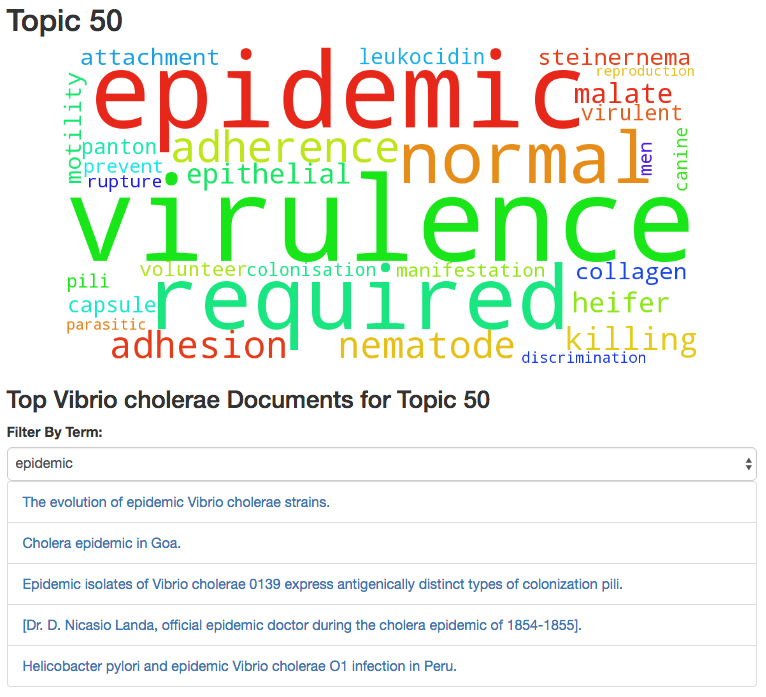
\includegraphics{fig01.eps}}
\caption{Caption, caption.}\label{fig:01}
\end{figure}

%\begin{figure}[!tpb]%figure2
%%\centerline{\includegraphics{fig02.eps}}
%\caption{Caption, caption.}\label{fig:02}
%\end{figure}

Text Text Text Text Text Text  Text Text Text Text Text Text Text
Text Text  Text Text Text Text Text Text.
Figure~2\vphantom{\ref{fig:02}} shows that the above method  Text
Text Text Text  Text Text Text Text Text Text  Text Text.
\citealp{Boffelli03} might want to know about  text text text text
Text Text Text Text Text Text  Text Text Text Text Text Text Text
Text Text  Text Text Text Text Text Text.
Figure~2\vphantom{\ref{fig:02}} shows that the above method  Text
Text Text Text  Text Text Text Text Text Text  Text Text.
\citealp{Boffelli03} might want to know about  text text text text
Text Text Text Text Text Text Text Text Text Text Text Text Text
Text Text  Text Text Text Text Text Text.
Figure~2\vphantom{\ref{fig:02}} shows that the above method  Text
Text Text Text  Text Text Text Text Text Text  Text Text.
\citealp{Boffelli03} might want to know about  text text text text


\subsection{Test1}

Text Text Text Text Text Text  Text Text Text Text Text Text Text
Text Text  Text Text Text Text Text Text.
Figure~2\vphantom{\ref{fig:02}} shows that the above method  Text
Text Text Text  Text Text Text Text Text Text  Text Text.
\citealp{Boffelli03} might want to know about  text text text text
Text Text Text Text Text Text  Text Text Text Text Text Text Text
Text Text  Text Text Text Text Text Text.
Figure~2\vphantom{\ref{fig:02}} shows that the above method  Text
Text Text Text  Text Text Text Text Text Text  Text Text.
\citealp{Boffelli03} might want to know about  text text text text
Text Text Text Text Text Text Text Text Text Text Text Text Text
Text Text  Text Text Text Text Text Text.
Figure~2\vphantom{\ref{fig:02}} shows that the above method  Text
Text Text Text  Text Text Text Text Text Text  Text Text.
\citealp{Boffelli03} might want to know about  text text text text





\section{Discussion}

Text Text Text Text Text Text  Text Text Text Text Text Text Text
Text Text  Text Text Text Text Text Text.
Figure~2\vphantom{\ref{fig:02}} shows that the above method  Text
Text Text Text  Text Text Text Text Text Text  Text Text.
\citealp{Boffelli03} might want to know about  text text text text
Text Text Text Text Text Text  Text Text Text Text Text Text Text
Text Text  Text Text Text Text Text Text.
Figure~2\vphantom{\ref{fig:02}} shows that the above method  Text
Text Text Text  Text Text Text Text Text Text  Text Text.
\citealp{Boffelli03} might want to know about  text text text text
Text Text Text Text Text Text Text Text Text Text.




Table~\ref{Tab:01} shows that Text Text Text Text Text  Text Text
Text Text Text Text. Figure~2\vphantom{\ref{fig:02}} shows that
the above method Text Text. Text Text Text  Text Text Text Text
Text Text. Figure~2\vphantom{\ref{fig:02}} shows that the above
method Text Text. Text Text Text  Text Text Text Text Text Text.
Figure~2\vphantom{\ref{fig:02}} shows that the above method Text
Text.









%%%%%%%%%%%%%%%%%%%%%%%%%%%%%%%%%%%%%%%%%%%%%%%%%%%%%%%%%%%%%%%%%%%%%%%%%%%%%%%%%%%%%
%
%     please remove the " % " symbol from \centerline{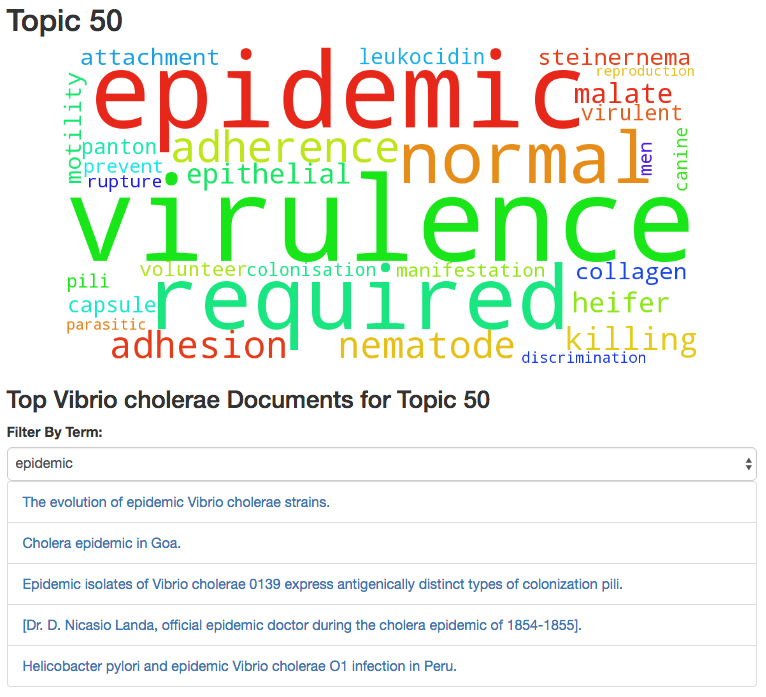
\includegraphics{fig01.eps}}
%     as it may ignore the figures.
%
%%%%%%%%%%%%%%%%%%%%%%%%%%%%%%%%%%%%%%%%%%%%%%%%%%%%%%%%%%%%%%%%%%%%%%%%%%%%%%%%%%%%%%






\section{Conclusion}

(Table~\ref{Tab:01}) Text Text Text Text Text Text  Text Text Text
Text Text Text Text Text Text  Text Text Text Text Text Text.
Figure~2\vphantom{\ref{fig:02}} shows that the above method  Text
Text Text Text  Text Text Text Text Text Text  Text Text.
\citealp{Boffelli03} might want to know about  text text text text
Text Text Text Text Text Text  Text Text Text Text Text Text Text
Text Text  Text Text Text Text Text Text.
Figure~2\vphantom{\ref{fig:02}} shows that the above method  Text
Text Text Text  Text Text Text Text Text Text  Text Text.
\citealp{Boffelli03} might want to know about  text text text text
Text Text Text Text Text Text Text Text Text Text Text Text Text
Text Text  Text Text Text Text Text Text.
Figure~2\vphantom{\ref{fig:02}} shows that the above method  Text
Text Text Text  Text Text Text Text Text Text  Text Text.



Text Text Text Text Text Text  Text Text Text Text Text Text Text
Text Text  Text Text Text Text Text Text.
Figure~2\vphantom{\ref{fig:02}} shows that the above method  Text
Text Text Text  Text Text Text Text Text Text  Text Text.
\citealp{Boffelli03} might want to know about  text text text text

\begin{enumerate}
\item this is item, use enumerate
\item this is item, use enumerate
\item this is item, use enumerate
\end{enumerate}

Text Text Text Text Text Text Text Text Text Text Text Text Text
Text Text Text Text Text Text Text Text.
Figure~2\vphantom{\ref{fig:02}} shows\vadjust{\pagebreak} that the
above method  Text Text Text Text Text Text Text Text Text Text
Text Text.  \citealp{Boffelli03} might want to know about text
text text text Text Text Text Text Text Text  Text Text Text Text
Text Text Text Text Text Text Text Text Text Text Text.
Figure~2\vphantom{\ref{fig:02}} shows that the above method  Text
Text Text Text Text Text Text Text Text Text  Text Text.
\citealp{Boffelli03} might want to know about text text text text
Text Text Text Text Text Text  Text Text Text Text Text Text Text
Text Text Text Text Text Text Text\break Text.


Text Text Text Text Text Text  Text Text Text Text Text Text Text
Text Text  Text Text Text Text Text Text.
Figure~2\vphantom{\ref{fig:02}} shows that the above method  Text
Text Text Text\vspace*{-10pt}


\section*{Acknowledgements}

Text Text Text Text Text Text  Text Text.  \citealp{Boffelli03} might want to know about  text
text text text\vspace*{-12pt}

\section*{Funding}

This work has been supported by the... Text Text  Text Text.\vspace*{-12pt}

%\bibliographystyle{natbib}
%\bibliographystyle{achemnat}
%\bibliographystyle{plainnat}
%\bibliographystyle{abbrv}
%\bibliographystyle{bioinformatics}
%
%\bibliographystyle{plain}
%
%\bibliography{Document}


\begin{thebibliography}{}

\bibitem[Bofelli {\it et~al}., 2000]{Boffelli03}
Bofelli,F., Name2, Name3 (2003) Article title, {\it Journal Name}, {\bf 199}, 133-154.

\bibitem[Bag {\it et~al}., 2001]{Bag01}
Bag,M., Name2, Name3 (2001) Article title, {\it Journal Name}, {\bf 99}, 33-54.

\bibitem[Yoo \textit{et~al}., 2003]{Yoo03}
Yoo,M.S. \textit{et~al}. (2003) Oxidative stress regulated genes
in nigral dopaminergic neurnol cell: correlation with the known
pathology in Parkinson's disease. \textit{Brain Res. Mol. Brain
Res.}, \textbf{110}(Suppl. 1), 76--84.

\bibitem[Lehmann, 1986]{Leh86}
Lehmann,E.L. (1986) Chapter title. \textit{Book Title}. Vol.~1, 2nd edn. Springer-Verlag, New York.

\bibitem[Crenshaw and Jones, 2003]{Cre03}
Crenshaw, B.,III, and Jones, W.B.,Jr (2003) The future of clinical
cancer management: one tumor, one chip. \textit{Bioinformatics},
doi:10.1093/bioinformatics/btn000.

\bibitem[Auhtor \textit{et~al}. (2000)]{Aut00}
Auhtor,A.B. \textit{et~al}. (2000) Chapter title. In Smith, A.C.
(ed.), \textit{Book Title}, 2nd edn. Publisher, Location, Vol. 1, pp.
???--???.

\bibitem[Bardet, 1920]{Bar20}
Bardet, G. (1920) Sur un syndrome d'obesite infantile avec
polydactylie et retinite pigmentaire (contribution a l'etude des
formes cliniques de l'obesite hypophysaire). PhD Thesis, name of
institution, Paris, France.

\end{thebibliography}
\end{document}
